\documentclass[10pt]{article}
\usepackage[utf8]{inputenc}
\usepackage[T1]{fontenc}
\usepackage{graphicx}
\usepackage{float}
\usepackage{hyperref}

\usepackage{indentfirst} % To indent first paragraph after a section

% Main title of the file
\title{\vspace{-3cm}Development of a Virtual Card Prototype for the University of Porto}
\date{}

\begin{document}
\maketitle

\section{Requirements and Functionalities Analysis}

\subsection{General Objective}
Development of a prototype for the virtual card of the University of Porto (U.Porto) with NFC technology. This virtual card will reapply the functionalities of the physical card, allowing its use through a digital Wallet integrated into mobile devices.

\subsection{Actors}
The primary users of this system encompass a broad spectrum of the University of Porto community members who are current holders of a physical institutional card. This includes but is not limited to students, faculty members, administrative and support staff, and other university personnel. The system is designed to cater to the diverse needs of this wide-ranging group, providing a seamless transition to a more digital and convenient form of access and identification across university services and facilities. Each actor, regardless of their specific role within the university, stands to benefit from the enhanced convenience, security, and efficiency offered by the virtual card system.

\subsection{Requirements Gathering}
\begin{itemize}
  \item Users will have access to their virtual card through a mobile digital Wallet.
  \item An application will be developed that will enable users to acquire a certificate for their card, provided they authenticate correctly.
  \item The system must include a robust and secure mechanism for generating and issuing cryptographic credentials. This feature should ensure the integrity and authenticity of digital certificates used for user authentication.
  \item System administrators should have a control panel that allows them to manage the system and perform various operations.
  \item Users will be able to report problems or suggest improvements in the application through an implemented feedback system (suggestion).
  \item Internally, the development of the application, along with all auxiliary components, will be thoroughly documented and tested using unit tests. This ensures the application functions correctly and facilitates a clear understanding of the various developed components that make up the final product.
\end{itemize}

\subsection{Use Case: Acquisition of the Virtual Card}
Context: A member of the University of Porto seeks to transition from frequently using their physical card to adopting a virtual version. The primary objective is to reduce the necessity of carrying a physical card. To achieve this, the member must securely obtain the virtual card through a digital process that ensures authentication and verification.

\subsubsection{Steps}
\begin{enumerate}
  \item Application Access: The user initiates the transition by accessing a dedicated application designed for the digital credential issuance process. The specific application to be used is to be determined.
  
  \item User Authentication: Upon entering the application, the user authenticates themselves using their University of Porto credentials. Alternative authentication methods may be considered for implementation to ensure security and ease of access.
  
  \item Virtual Card Issuance: Following successful authentication, the user formally requests their virtual card. The application then generates and assigns a digital certificate, effectively issuing the virtual card.
\end{enumerate}

Result: The user successfully acquires their NFC-enabled virtual card, fully equipped with the necessary cryptographic credentials for secure identification and access within the University of Porto's ecosystem.

\subsection{Use Case: Utilizing the Virtual Card through a Digital Wallet at the University of Porto}
Context: A university member is now equipped with their NFC-enabled virtual card stored within a digital wallet app on their mobile device. They aim to utilize this virtual card for various campus services that previously required a physical card.

\subsubsection{Steps}
\begin{enumerate}
  \item Opening the Digital Wallet: The user unlocks their mobile device and opens the digital wallet application where the virtual card is securely stored.
  
  \item Selecting the Virtual Card: Within the digital wallet, the user selects the U.Porto virtual card, preparing it for use by activating the NFC feature on their device.
  
  \item Accessing Campus Services: The user approaches an NFC-enabled terminal and brings their device close to the NFC reader.
  
  \item Transaction Confirmation: The NFC-enabled terminal reads the virtual card's cryptographic credentials, verifies the user's identity and permissions, and processes the transaction or grants access accordingly.
  
  \item Visual/Audible Confirmation: Upon successful verification and transaction completion, the terminal provides a visual and/or audible confirmation to the user. The digital wallet may also display a transaction summary or access granted notification.
\end{enumerate}

Result: The university member seamlessly utilizes their NFC-enabled virtual card for a wide range of services across campus, enjoying a convenient and secure experience.

\section{Market Study for Digital Wallets}

\subsection{Introduction}

In recent years, digital wallets have emerged as a dominant trend, providing users with the convenience of carrying and using their payment cards, along with a variety of other documents, such as ID cards and transportation tickets, in a completely digital way. By storing these documents securely and encrypted, these applications not only offer convenience, but also guarantee the security of users' sensitive data.

Additionally, digital wallets constitute a greener and more sustainable approach, as they reduce the need for physical cards and paper, contributing to the preservation of the environment.

Given our lack of prior knowledge, we decided to carry out an in-depth study of the market to identify the best possible approach. In this regard, we analyzed various applications that use technologies such as NFC (Near Field Communication), digital wallets and other projects from other universities that have also migrated from physical cards to virtual cards. This comprehensive research allowed us to gain valuable knowledge about current trends and effective practices, providing a solid basis for the design and implementation of our own project.

\subsection{NFC}

NFC is a technology that allows the exchange of information between compatible devices over a very short distance, usually up to 4cm. Devices with this technology, when placed close together, are able to create a radio frequency field that enables them to communicate.

\subsubsection{Main modes of operation}
\begin{itemize}
    \item \textbf{Reader/Writer mode: } In this mode, the NFC device functions as a reader that can interact with passive NFC tags (such as cards or labels) to read or write information on them. This mode is used for contactless payments, access to facilities, etc...
    \item \textbf{Card Emulation Mode: } In this mode, the NFC device works as if it were an NFC card, allowing it to be detected and read by other devices, such as payment terminals or facility access readers;
    \item \textbf{Peer-to-Peer mode: } In this mode, two NFC devices can exchange information bidirectionally. This allows direct communication between the devices, facilitating data transfer, such as file exchange, information sharing or even mobile payments between the devices.
\end{itemize}

Of the existing operating modes, Card Emulation Mode is particularly relevant, as it allows mobile devices to act as
as university cards, facilitating access to university services and facilities, and even use
even use for digital student identification. It also allows for payments, something that should be possible with our cards.
In order to better understand how to implement these modes, we decided to analyze in which situations NFC is used and in which cases it is most effective:

\begin{itemize}
    \item \textbf{MB Way:} A mobile payment application that allows you to carry out various transactions using your cell phone. It uses NFC to make payments in physical stores, so all you have to do is bring your phone close to the scanning terminal.
    \item \textbf{Digital Mobile Key:} A digital authentication application that allows Portuguese citizens to access various online services with their cell phone. It uses NFC to authenticate the user in online services, simply by bringing the cell phone close to the reader terminal.
    \item \textbf{App Anda:} An application for paying journeys on public transport in the Porto Metropolitan Area. It uses NFC to pay for journeys, simply by bringing the card close to the validator.
\end{itemize}


\subsection{Digital Wallets}

Digital wallets are virtual platforms that allow users to store and manage financial and personal information electronically. They facilitate payments online and in physical stores, offering convenience and security. Digital wallets are becoming popular due to the convenience of storing multiple cards and the additional protection against fraud.

\subsubsection{Use Cases}

\begin{itemize}
    \item \textbf{University card:} Users can use their virtual card as if it were their physical card, speeding up the process of using university services;
    \item \textbf{Payments in physical stores:} Users can pay for their purchases in physical stores, using their virtual payment cards and avoiding the use of physical cards;
    \item \textbf{Identification:} The user can use their digital wallet to identify themselves when necessary;
    \item \textbf{Transport tickets:} The user can have a virtual transport pass, just like a transport ticket, avoiding the need to have a physical ticket;
\end{itemize}


Our application will be a digital wallet that will focus on the use cases of a university card and identification. Despite this, it won't differ much from other applications that use digital wallets for other purposes, so these can be used as examples. In order to develop a good implementation of a digital wallet, we analyzed some existing applications.

\subsubsection{Apple Wallet}
Apple Wallet is one of the most popular digital wallets. You can use it on Apple products other than your cell phone, such as the Apple Watch and iPad. In addition to the possibility of adding payment cards, Apple Wallet allows you to use Apple Pay, Apple's payment service that makes it easy to make payments in physical stores and online. However, this digital wallet is integrated with many other services that allow users to add loyalty cards, transport tickets and more.

In order to guarantee security for its users, cards such as loyalty cards, identification documents, among others, need a trusted certificate to be added to the digital wallet, ensuring that they are genuine.
Although payment cards in the Apple wallet also need to guarantee their eligibility, in these cards, the Apple wallet communicates with the card provider, guaranteeing the legitimacy of the card and users authenticate themselves to ensure that they are the owners of the card. To minimize the risk of compromised information theft, a unique token, which stores the card information, is generated and encrypted on the device's Secure Element Chip, ensuring that the card information is not shared.

\begin{figure}[H]
    \centering
    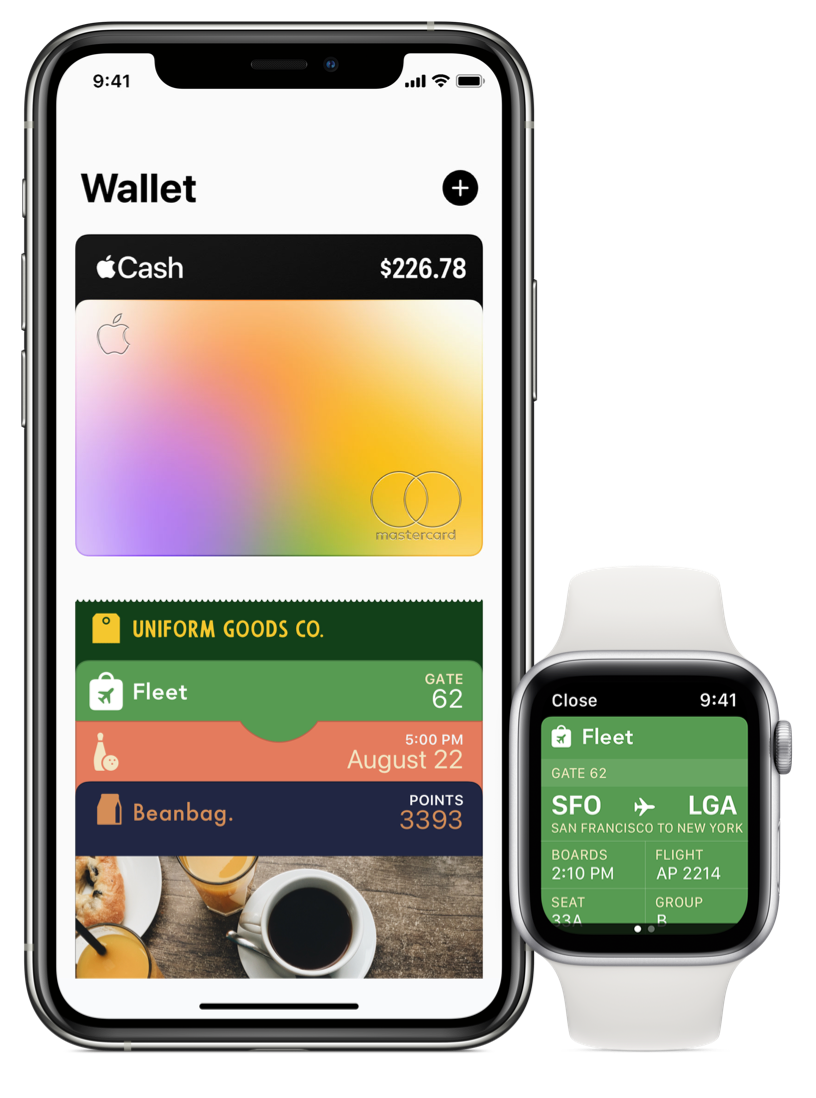
\includegraphics[width=0.5\textwidth]{report-images/apple-wallet.png}
    \caption{Graphic interface of Apple Wallet}
    \label{fig:fig-1}
\end{figure}

\subsection{Google Wallet}
Like Apple Wallet, Google Wallet is one of the most popular digital wallets. Like the previous one, it allows you to add different types of cards and can be used on devices other than just cell phones. In addition, Google Wallet allows the use of Google Pay, a service that guarantees the user the possibility of making payments.
In order to certify the eligibility of the cards it adds, Google Wallet needs the card providers to have used a legitimate certificate. In the case of cards used for payments, Google Wallet communicates with the user's bank and verifies their identity through user authentication. As with Apple Wallet, in order to guarantee the security of payment card information, a unique token is used that encrypts the card information.

\begin{figure}[H]
    \centering
    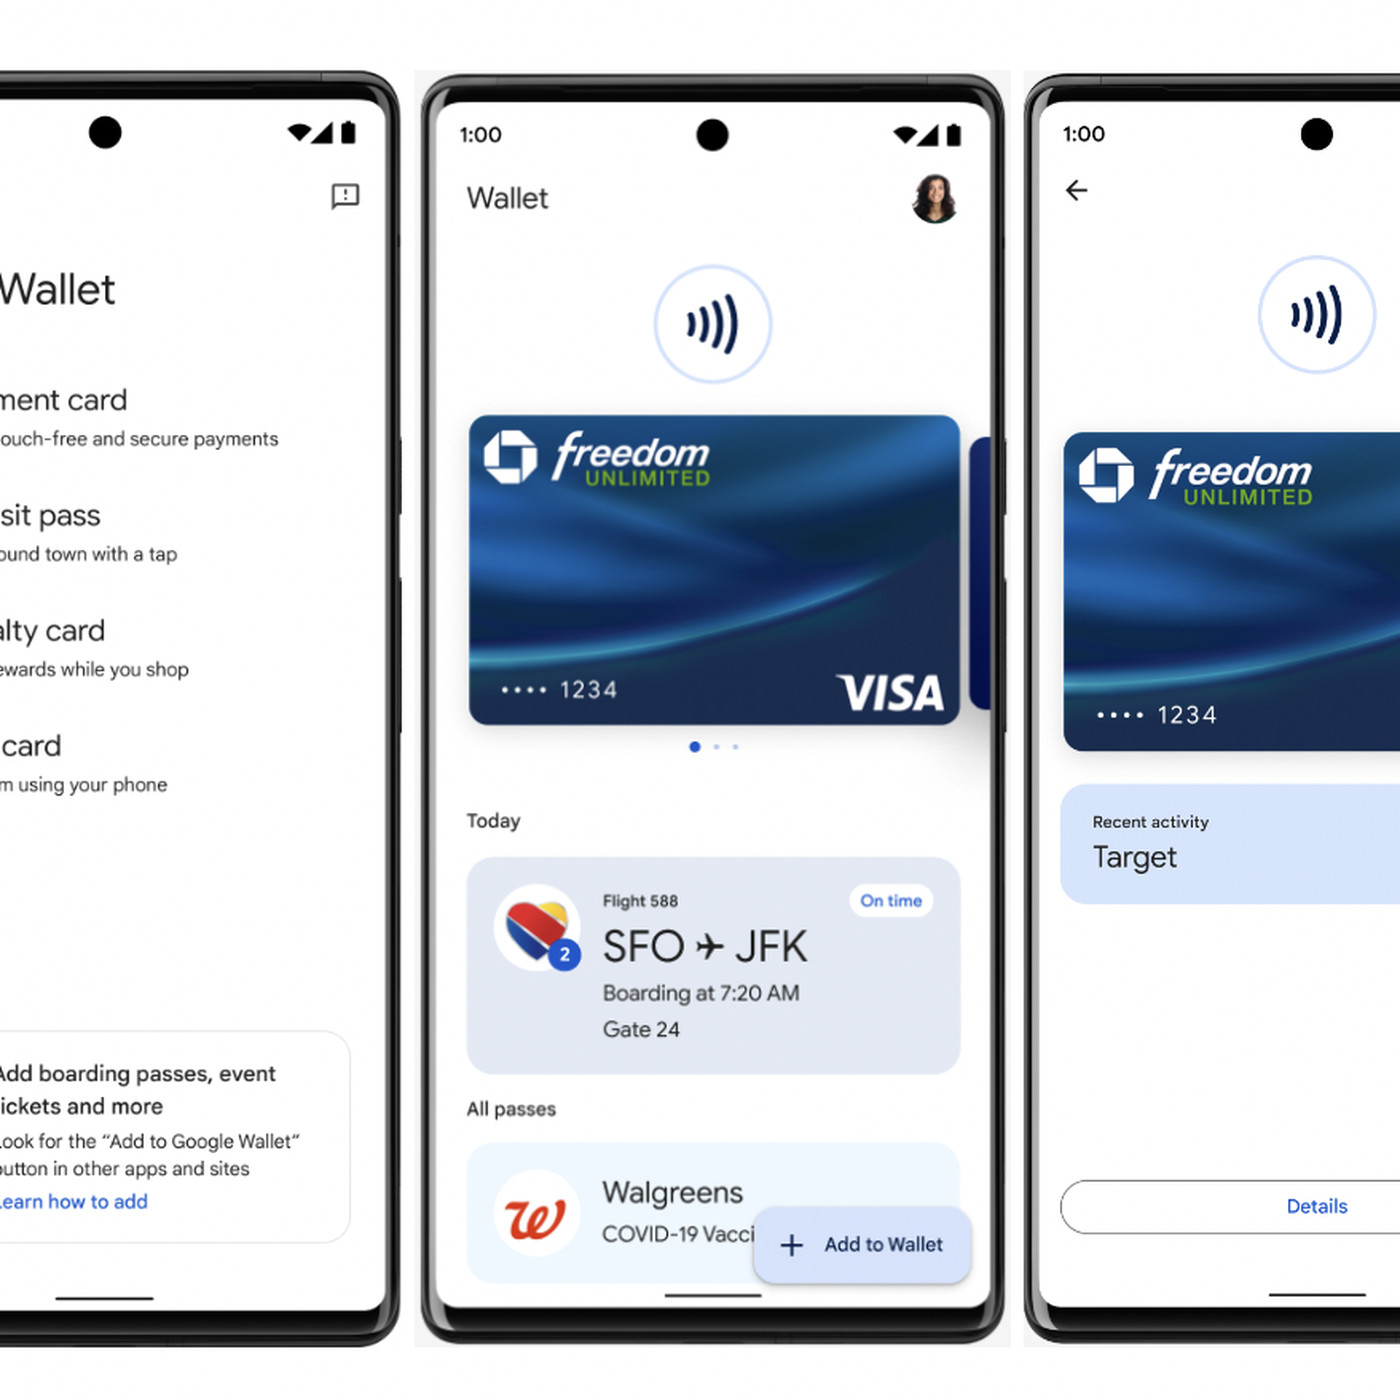
\includegraphics[width=0.5\textwidth]{report-images/google-wallet.png}
    \caption{Graphic interface of Google Wallet}
    \label{fig:fig-2}
\end{figure}

\subsection{Panorama of the Education and University Market}
As part of a preliminary study into the higher education sector, we have dedicated ourselves to exploring the current state of innovation, with particular attention to the institutions
that have already implemented the virtual student card. This interest stems from the
growing trend towards the digitization of academic services, with the aim of both
optimizing processes and improving the student experience.

\subsubsection{International Adoption of Digital Student Cards}
Google Wallet already facilitates the use of digital student cards at
several colleges located in Australia, the United States and Canada, indicating
a significant advance in the adoption of this technology on a global scale. Among the
pioneering institutions in this initiative are:

\begin{itemize}
    \item \textbf{Monash University, Australia: }Monash University stands out for its
          innovation with M-Pass, which integrates with Google Wallet and Apple Wallet.
          This system not only reflects adaptability to emerging technological
          trends, but also highlights the potential for transforming academic
          academic services through digitalization. The acquisition of M-Pass requires
          that students authenticate themselves with their academic credentials and
          validate their identity by submitting an official document (passport or driver's license). This process emphasizes security and
          authentication, which are fundamental to the success of such digital initiatives.
          Through the university's app, students can load credits
          to the card, although the full functionality of the card has not been
          fully specified.
    \item \textbf{University of York, Canada: }The YU-Card, implemented by the University of
          York, provides students with a practical way to access a wide range of
          university services and spaces. Unlike the M-Pass,
          the YU-Card is rechargeable via the university's website.
\end{itemize}

\subsubsection{European Perspectives}
In Europe, the European Student Card (ESC) initiative is set to offer a digital solution to higher education institutions participating in the Erasmus+ program by 2025. This initiative underscores a dedication to enhancing student mobility and integrating academic services through digital platforms. It represents a significant move towards the harmonization and streamlining of educational processes across Europe, facilitating a more unified and simplified academic experience for students.

\section{Perception of surroundings:}

\subsection{Introduction}

The main goal of our project is to make the card system at the University of Porto more sustainable and practical, through a digital wallet that will allow students and staff at the University of Porto to use their card via a mobile phone.
Considering that our target audience will be the academic community of the University of Porto, we decided to create and share a survey in order to understand what would be the best approach to develop our application and
to obtain knowledge about users' expectations of our application, as well as their familiarity with technology and their priorities in a digital wallet.

\subsection{Analysis of responses}


We obtained a total of 48 responses, all from students currently enrolled at a Higher Education Institution. Considering the target audience previously defined, this indicates that all the responses will be valuable, as they represent possible users of the application.

\begin{figure}[h]
    \centering
    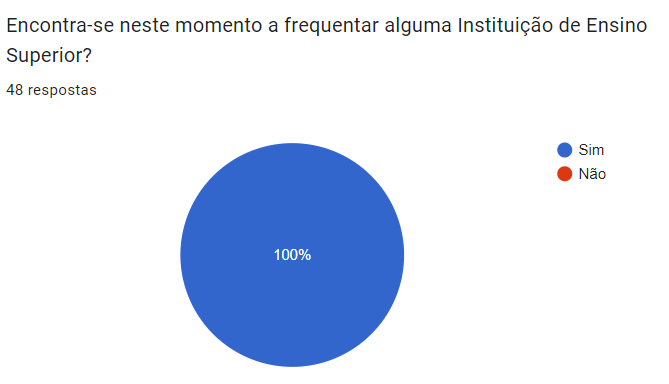
\includegraphics[width=0.7\textwidth]{report-images/questionaire1.png}
    \caption{Object of study}
    \label{fig:fig-3}
\end{figure}


\subsubsection{Frequency and use cases}

Around 60\% of users responded that they used their institutional card frequently, with the most used services being: \textbf{Access to the canteen} (~64\%), \textbf{Access to classrooms/cores} (50\%) and \textbf{Identification in tests/exams} (~44\%).
This suggests that it will be crucial to create a quickly accessible application for occasional, short-term use, as well as the possibility of it serving as a means of institutional identification for the user holding the virtual card.

\begin{figure}[h]
    \centering
    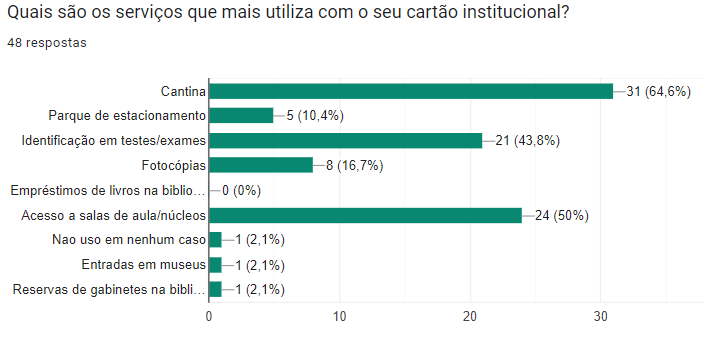
\includegraphics[width=0.9\textwidth]{report-images/questionaire2.png}
    \caption{Where do you use your card?}
    \label{fig:fig-4}
\end{figure}

\begin{figure}[h]
    \centering
    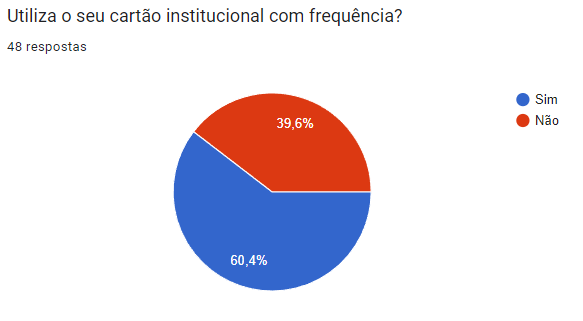
\includegraphics[width=0.9\textwidth]{report-images/questionaire3.png}
    \caption{Do you use your card frequently?}
    \label{fig:fig-5}
\end{figure}

\subsubsection{Previous experience with technologies}

All but one of the participants answered that they had previous experience with virtual cards, and of the 47 relevant answers, 35 (75\%) reported a very good experience using it. We therefore concluded that our target audience felt comfortable with the technologies used, which will allow us to use current applications that implement these functionalities as inspiration.
Through the survey, we were also able to analyze some of the difficulties that some participants had using similar applications:
\begin{itemize}
    \item \textbf Virtual card creation process
    \item \textbf Errors in carrying out the different operations using the application.
\end{itemize}


These difficulties allow us to conclude that we must make these processes intuitive and provide support to users.



\subsubsection{Expectations and suggestions}

According to the expectations of potential future users, we see a greater interest in the security of the application (77\%) as well as the convenience it will bring (71\%). We therefore need to focus on guaranteeing the security of the users' data and the convenience of using the solution to justify the possible replacement of the physical card in many cases.
We also noticed an interest in a simple interface for the application (52\%).

\begin{figure}[h]
    \centering
    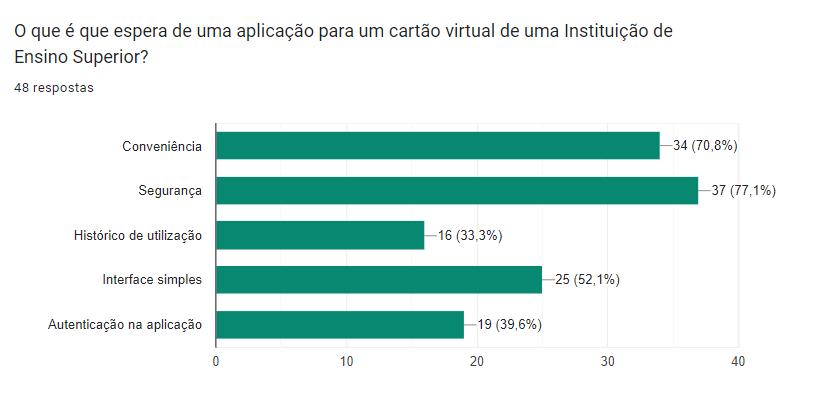
\includegraphics[width=1\textwidth]{report-images/questionaire4.png}
    \caption{What are your expectations for the application?}
    \label{fig:fig-6}
\end{figure}


\section{Low and High Level Mockups}

Prior to initiating the development process, we created comprehensive mockups that included both conceptual (high-level) and detailed (low-level) designs for the core pages of the web application. For the low-level mockups we included both desktop and mobile versions, we also made translations for the pages in english, but we did not include them in this report.

\subsection{Landing Page}

\begin{figure}[H]
  \centering
  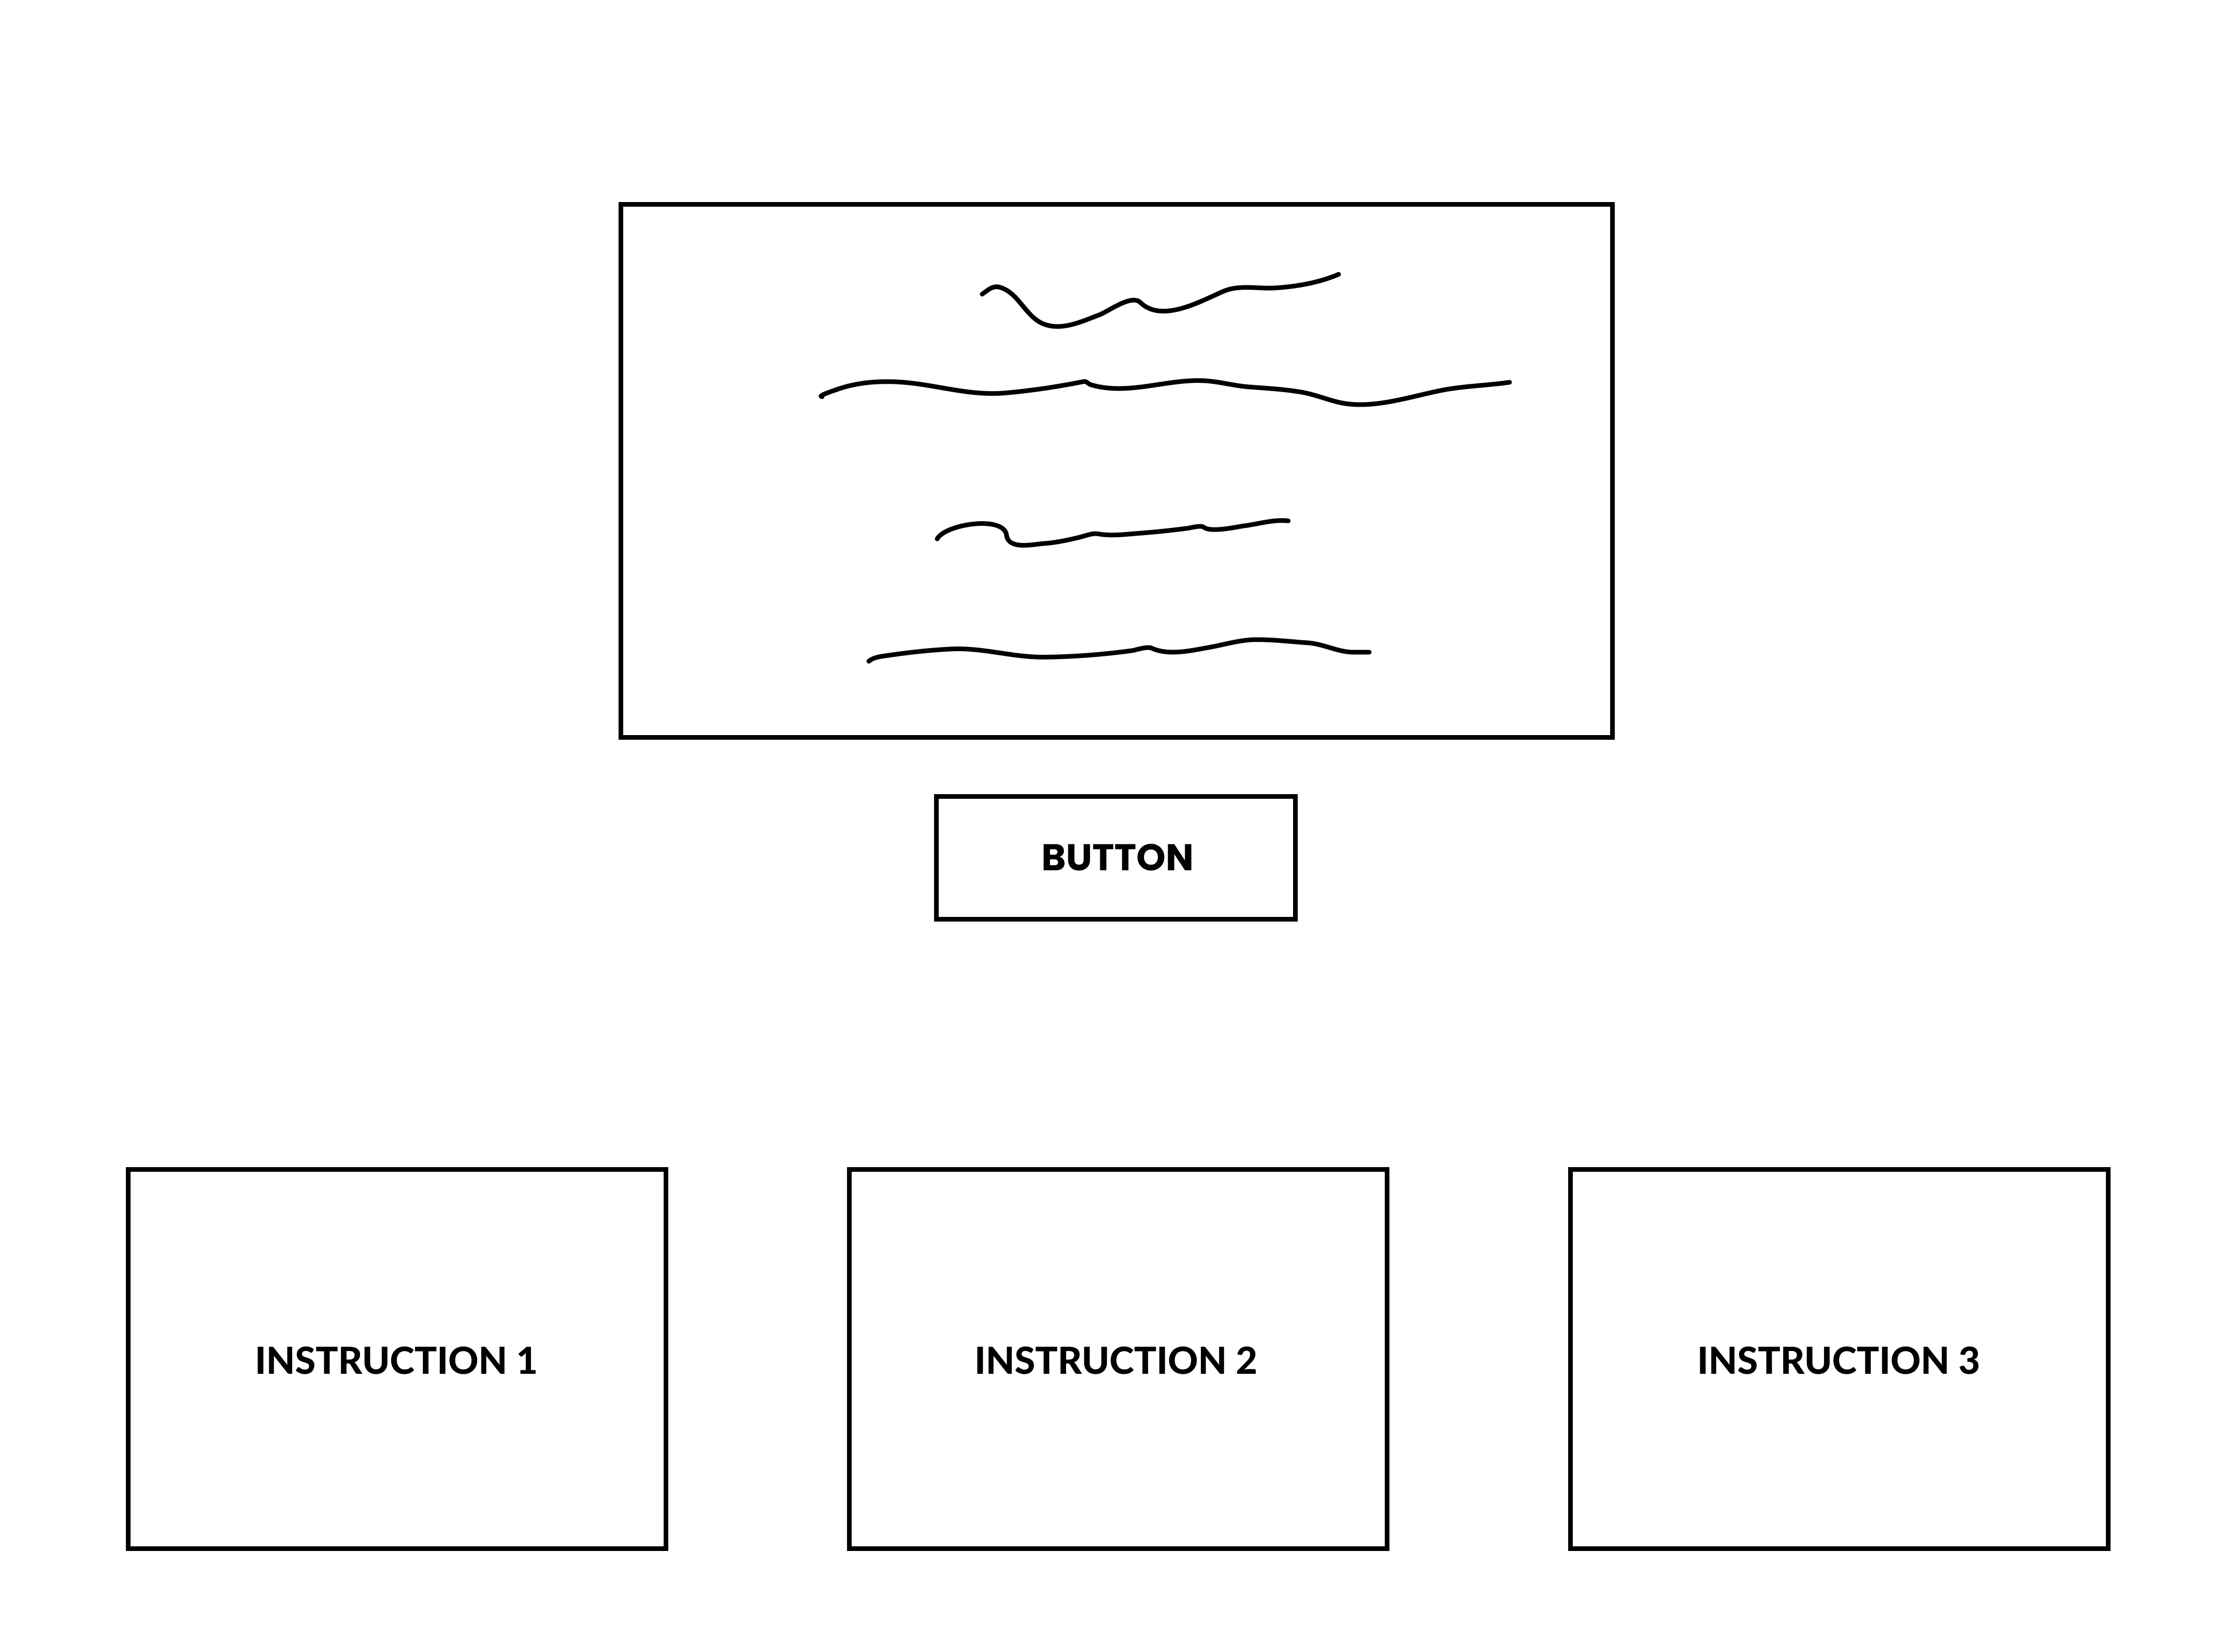
\includegraphics[width=1\linewidth]{report-images/landing-page-high-level.png}
  \caption{High level mockup of the landing page.}
  \label{fig:fig-7}
\end{figure}

\begin{figure}[H]
  \centering
  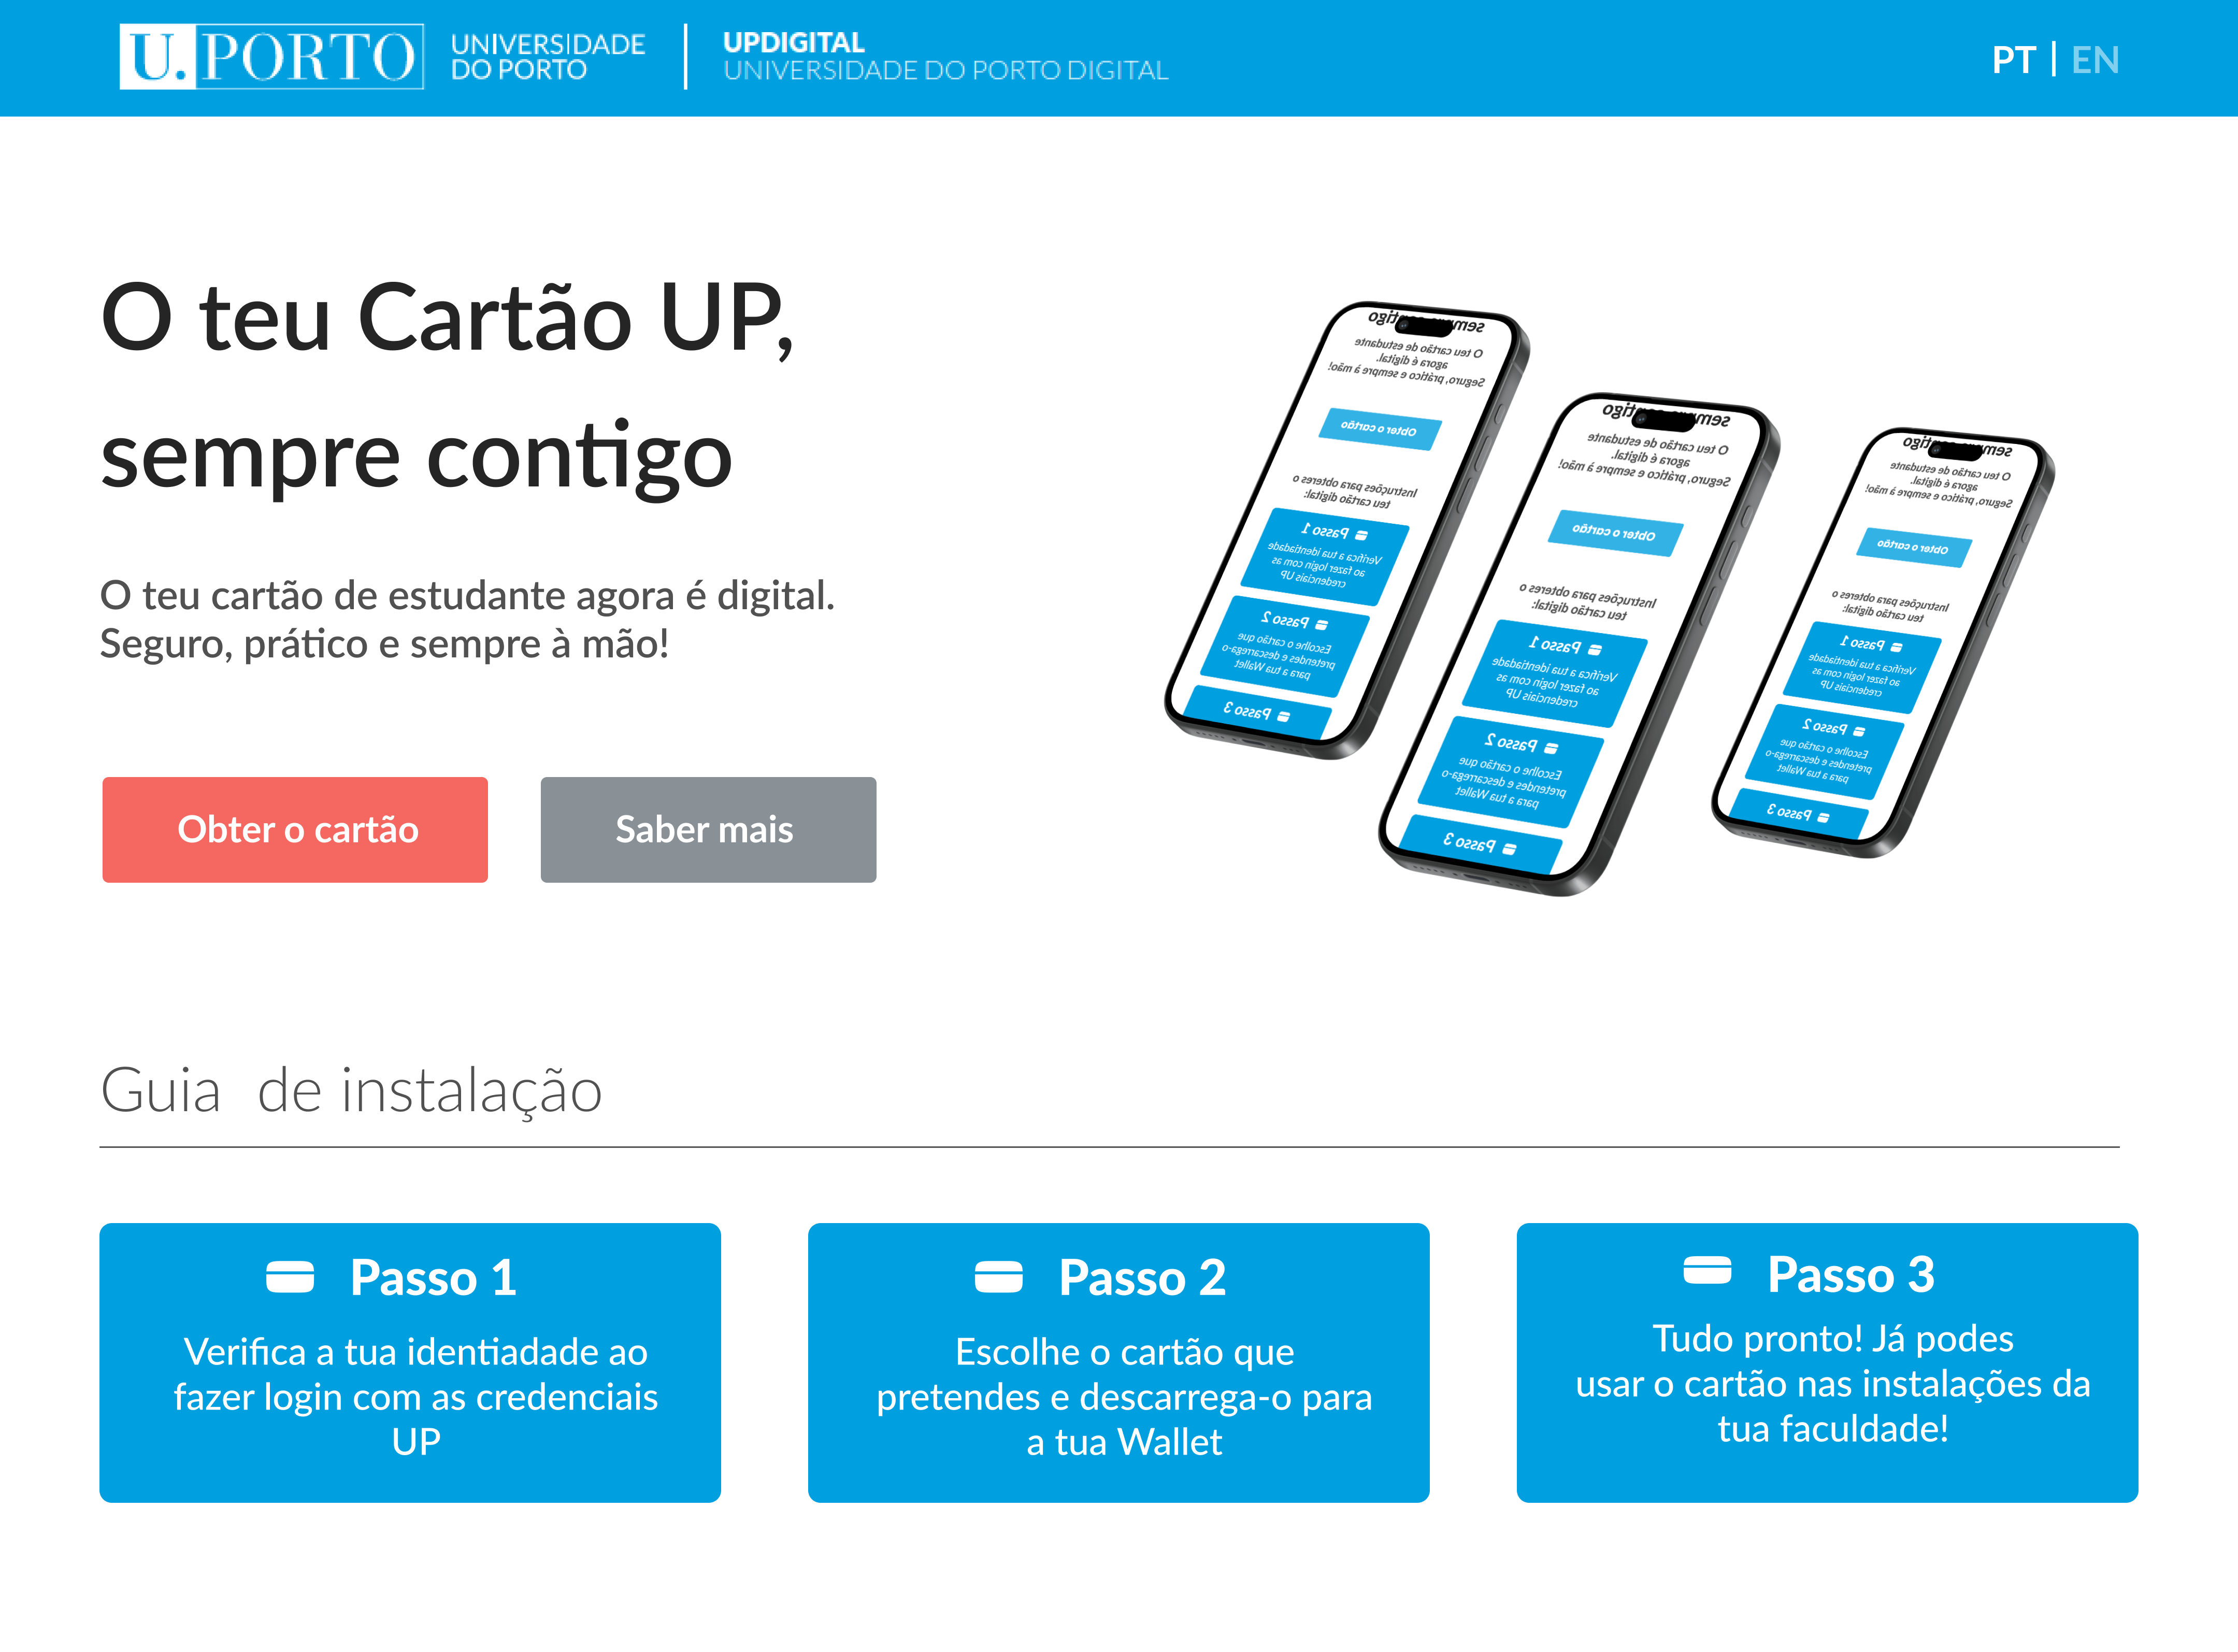
\includegraphics[width=1\linewidth]{report-images/landing-page-desktop.png}
  \caption{Low level mockup of the landing page - desktop version.}
  \label{fig:fig-8}
\end{figure}

\begin{figure}[H]
  \centering
  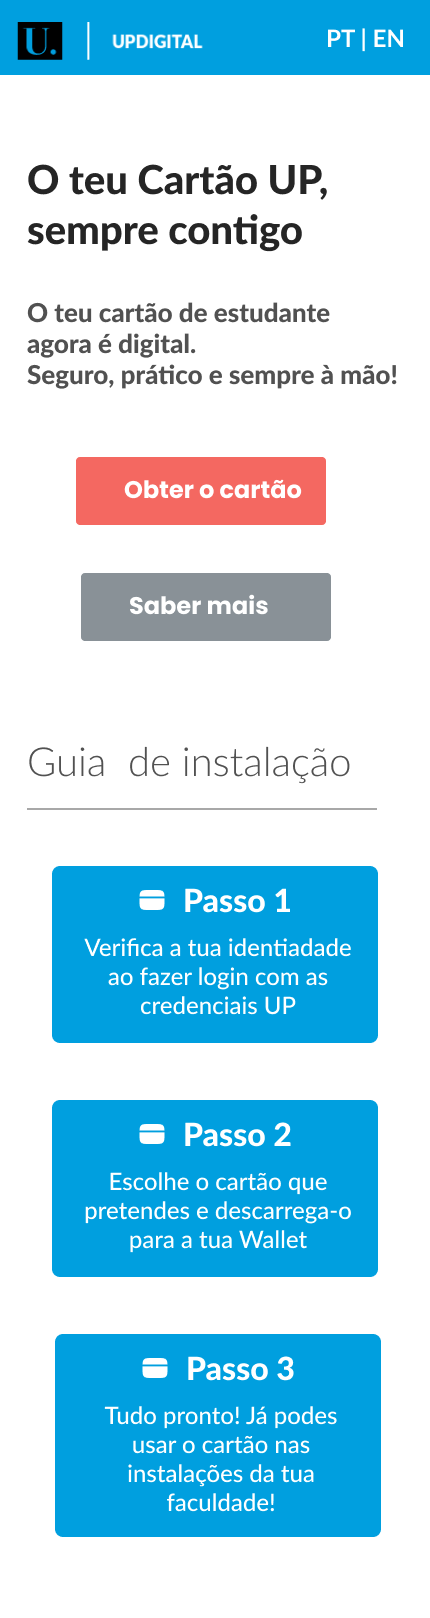
\includegraphics[width=0.25\linewidth]{report-images/landing-page-mobile.png}
  \caption{Low level mockup of the landing page - mobile version.}
  \label{fig:fig-9}
\end{figure}

\clearpage % Force all figures to be outputted before continuing

\subsection{Authentication Page}

\begin{figure}[H]
  \centering
  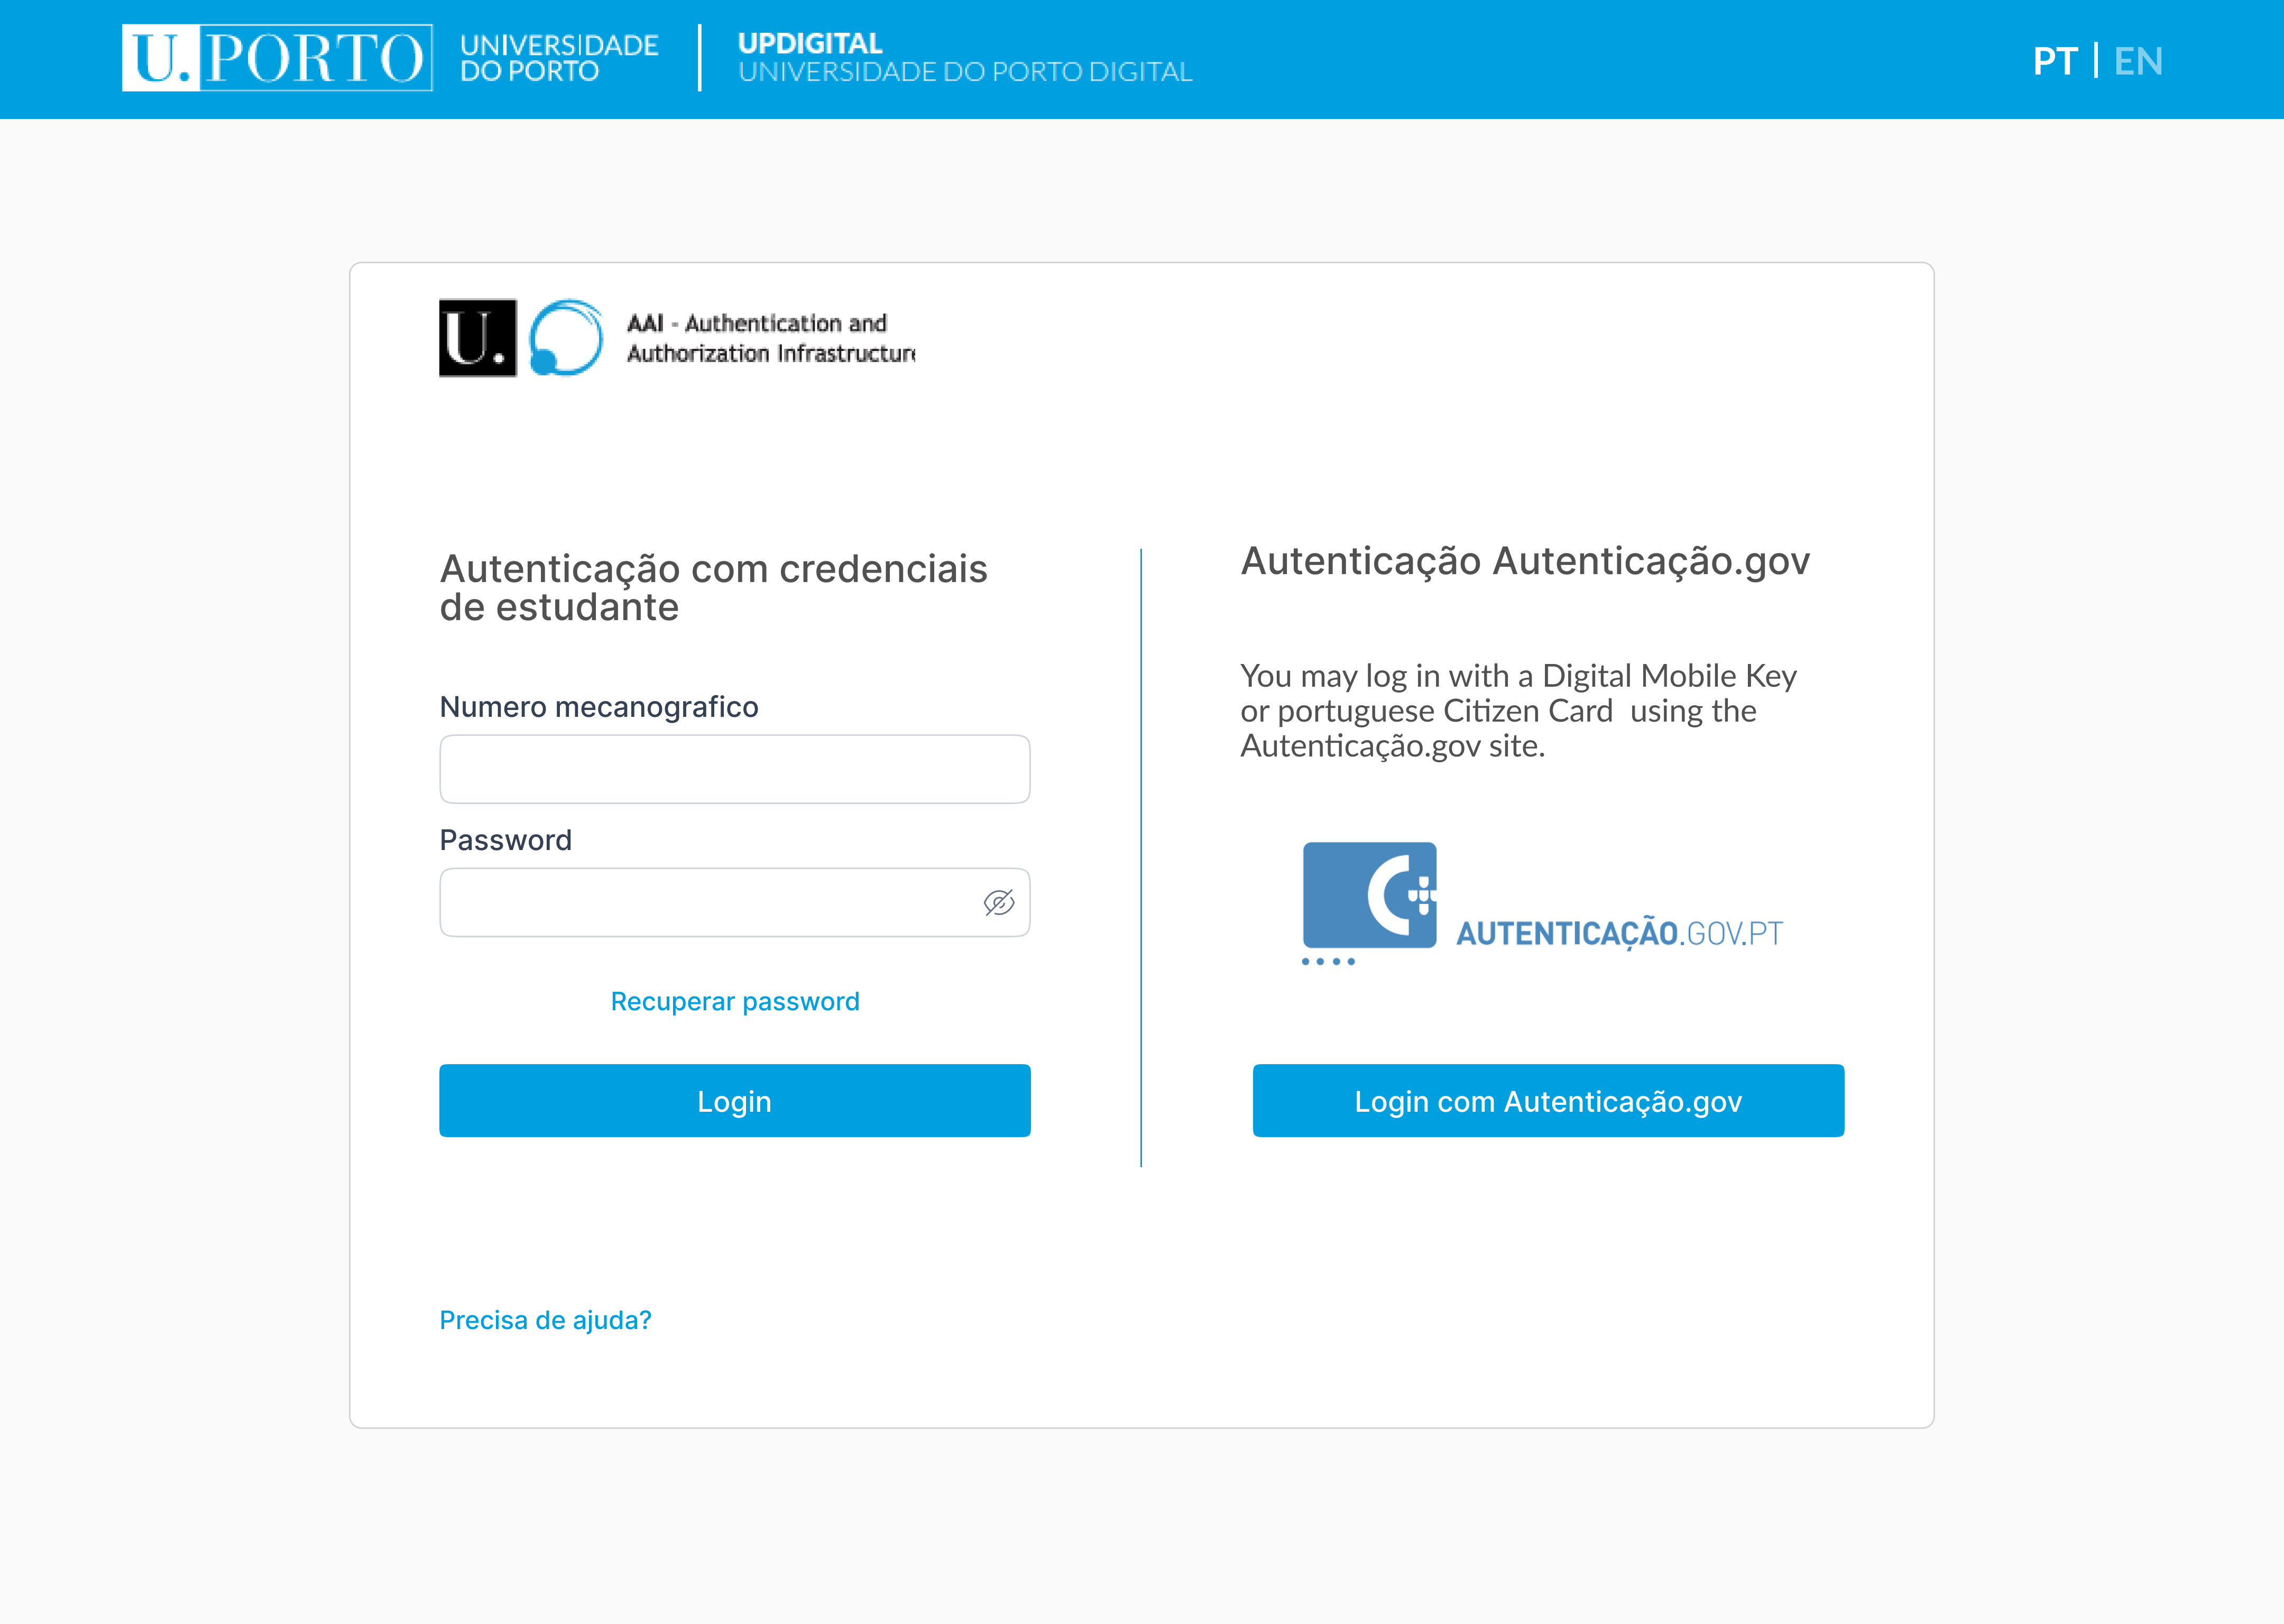
\includegraphics[width=1\linewidth]{report-images/authentication-page-desktop.png}
  \caption{Low level mockup of the authentication page - desktop version.}
  \label{fig:fig-10}
\end{figure}

\clearpage

\subsection{QRCode Page}

\begin{figure}[H]
  \centering
  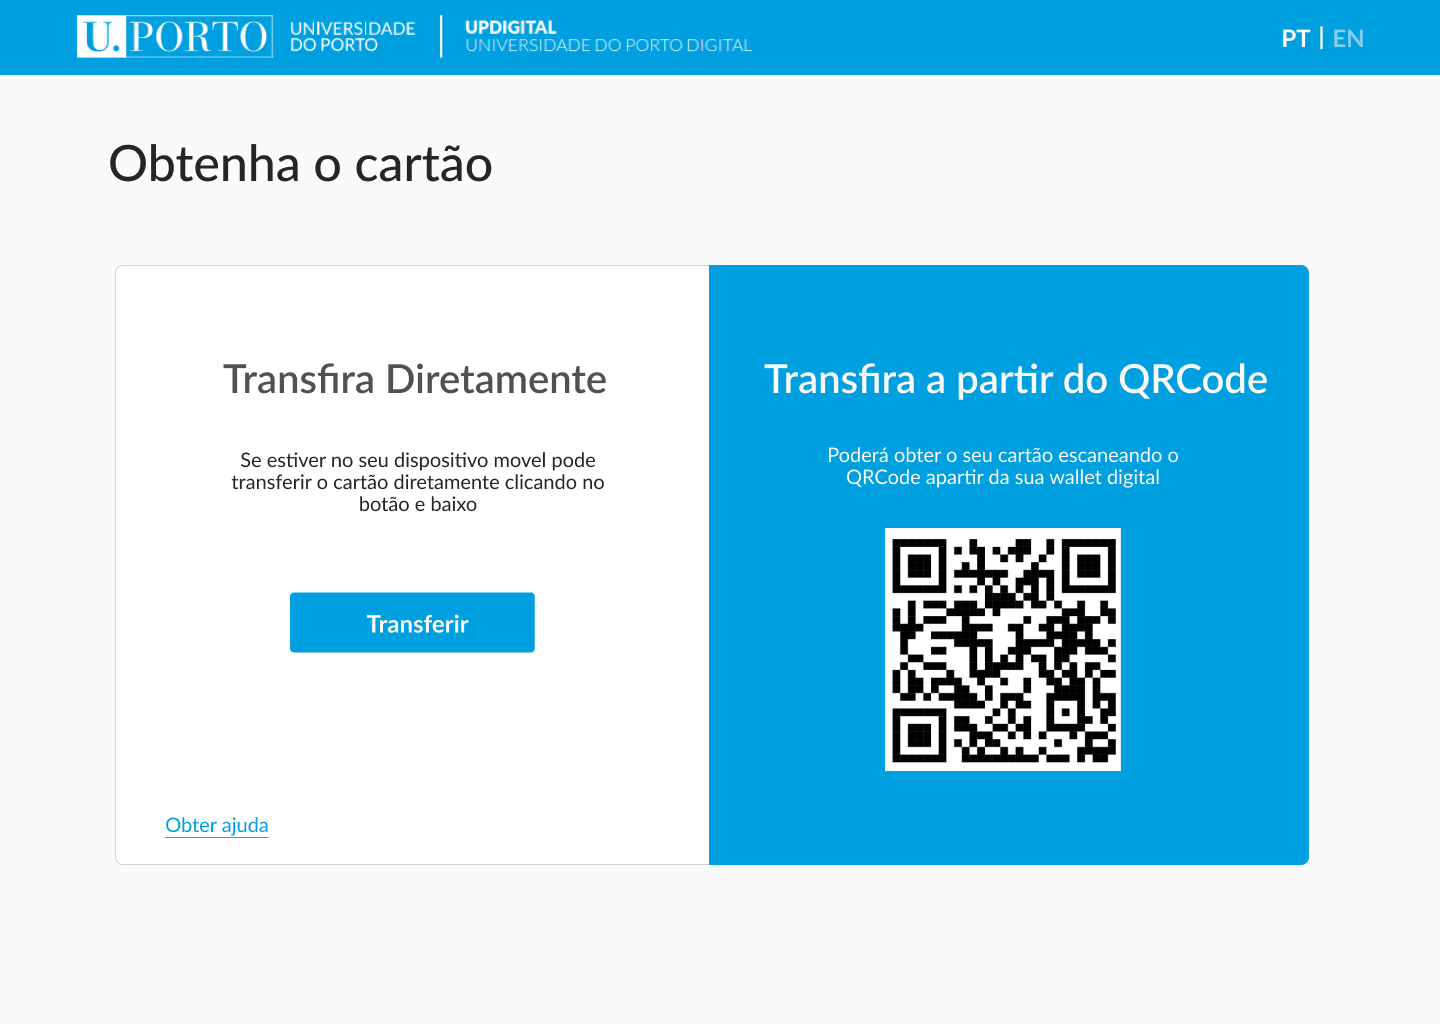
\includegraphics[width=1\linewidth]{report-images/qrcode-page-desktop.png}
  \caption{Low level mockup of the qrcode page - desktop version.}
  \label{fig:fig-11}
\end{figure}

\begin{figure}[H]
  \centering
  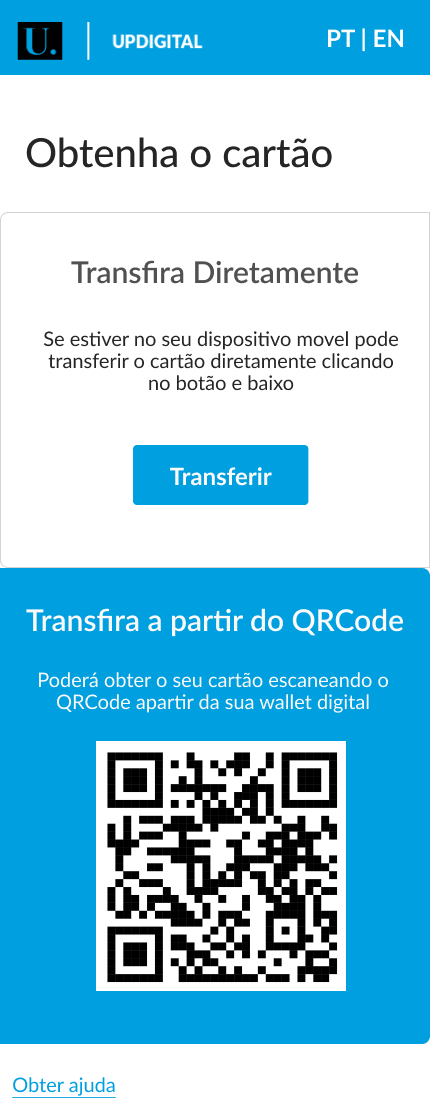
\includegraphics[width=0.25\linewidth]{report-images/qrcode-page-mobile.png}
  \caption{Low level mockup of the qrcode page - mobile version.}
  \label{fig:fig-12}
\end{figure}

\begin{thebibliography}{9}
  \bibitem{ApplePaycomponentsecurity}
  \textit{Apple Pay Component Security},
  \url{https://support.apple.com/guide/security/apple-pay-component-security-sec2561eb018/web}

  \bibitem{applewallet}
  \textit{Apple Wallet},
  \url{https://developer.apple.com/wallet/get-started/}

  \bibitem{applepay}
  \textit{Apple Pay},
  \url{https://support.apple.com/en-us/HT203027}

  \bibitem{genericPass}
  \textit{Generic Cards},
  \url{https://developers.google.com/wallet/generic}

  \bibitem{googlewallet}
  \textit{Google Wallet},
  \url{https://wallet.google/}

  \bibitem{googlepay}
  \textit{Google Pay},
  \url{https://developers.google.com/pay/issuers/tsp-integration/overview}

  \bibitem{monash}
  \textit{Monash University},
  \url{https://www.monash.edu/students/support/connect/id}

  \bibitem{york}
  \textit{York University},
  \url{https://www.yorku.ca/yucard/}

  \bibitem{esc}
  \textit{European Student Card},
  \url{https://erasmus-plus.ec.europa.eu/european-student-card-initiative/card/about}

  \bibitem{campusMobileWallet}
  \textit{Campus Mobile Wallet},
  \url{https://en.wikipedia.org/wiki/List_of_campus_identifications_in_mobile_wallets}

\end{thebibliography}

\end{document}
